%%%%%%%%%%%%%%%%%%%%%%%%%%%%%%%%%%%%%%%%%%%%%%%%%%%%%%%%%%%%%%%%%%%%%%%%%%%%%%%
\section{LTS Transformations}
\label{sec:lts-transformation:transformations}

In this section, we formalize refinement steps as transformations of networks of LTSs.
A network is transformed by transforming the individual process LTSs that constitute it and adding additional synchronization rules.

\subsection{Transformation Rules}
LTSs are transformed by applying transformation rules.
These rules are defined as follows.

\begin{definition}
\label{def:lts-transformation:transformationrule}
An LTS transformation rule $r = \transruletuple{r}$ consists of a left pattern LTS~$\Llts^r = \ltstuple{\Llts^r}$ and a right pattern LTS~$\Rlts^r = \ltstuple{\Rlts^r}$, with~$\initialstates{\Llts^r} = \initialstates{\Rlts^r} = (\states{\Llts^r} \cap \states{\Rlts^r})$.
\end{definition}

States $\states{\Llts^r} \cap \states{\Rlts^r}$, also referred to as the glue-states, are all initial and define how $\Rlts^r$ should replace $\Llts^r$.
All changes to an LTS are applied relative to these glue-states.
We call a rule~$r = \transruletuple{r}$ applicable on an LTS~$\graph$ iff there exists a match $m_r:\states{\Llts^r} \to \states\graph$ for which the following holds.

\clearpage

\begin{definition}
\label{def:lts-transformation:transmatch}
A transformation rule $r = \langle \Llts^r, \Rlts^r \rangle$ has a match~$m_r: \states{\Llts^r} \to \states{\graph}$ on an LTS~$\graph = \ltstuple{\graph}$ iff $m_r$ is injective and
\begin{enumerate}
\item $\forall s_1\xrightarrow{a}_{\Llts^r} s_2. m_r(s_1)\xrightarrow{a}_\graph m_r(s_2)$;
\item $\forall s_1 \in \states{\Llts^r} \setminus \states{\Rlts^r}, s_2 \in \states{\graph}:$
	\begin{itemize}
 	\item $m_r(s_1) \xrightarrow{a}_\graph s_2 \implies \exists s \in \states{\Llts^r}. s_1\xrightarrow{a} s \wedge m_r(s) = s_2$;
 	\item $s_2 \xrightarrow{a}_\graph m_r(s_1) \implies \exists s \in \states{\Llts^r}. s\xrightarrow{a} s_1 \wedge m_r(s) = s_2$.
	\end{itemize}
\end{enumerate}
\end{definition}

The second condition of Definition~\ref{def:lts-transformation:transmatch} is related to what are often called dangling edges.
In graph transformation, dangling edges (transitions) are usually removed as part of a transformation.
Here, we decide to make a rule non-applicable in case dangling transitions are present.
Otherwise, the effect of a transformation would be hard to predict based only on the rule itself, because it may cause states that are not present in the rule to become unreachable.

\begin{figure}[hbt]
\centering
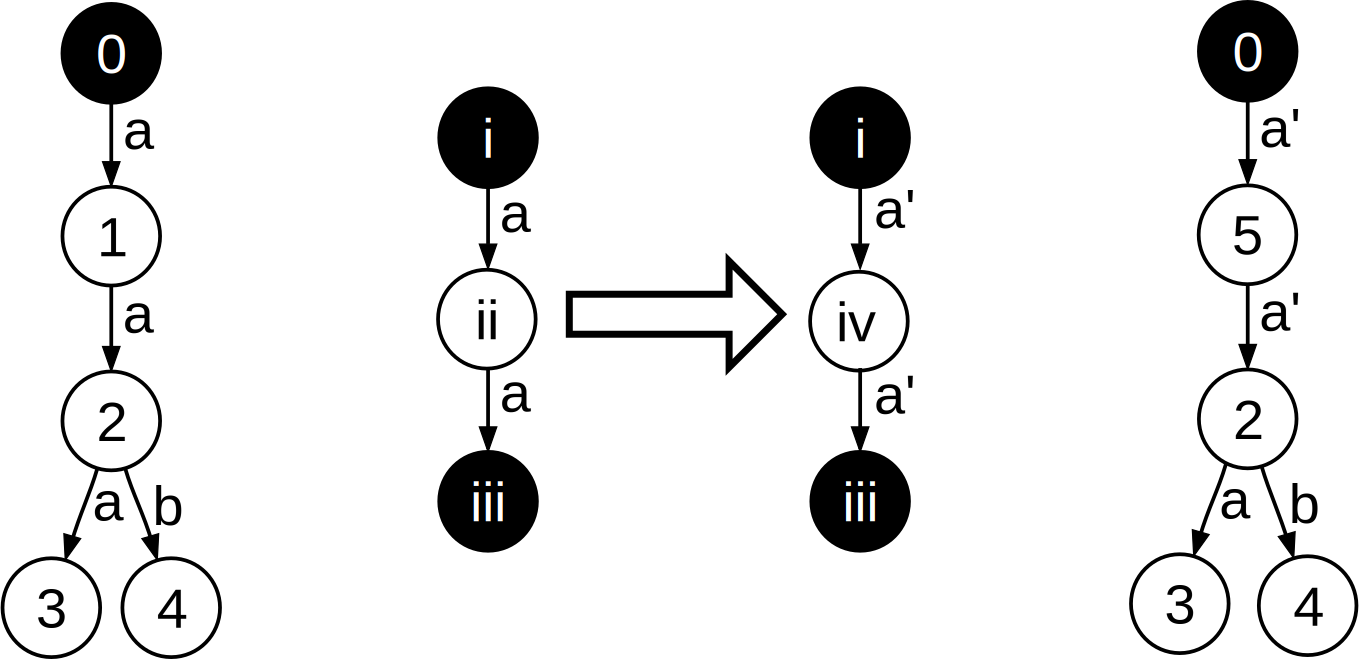
\includegraphics[scale=0.19]{lts-transformation/figs/matching}
\caption{Transformation rule matching}
\label{fig:lts-transformation:match}
\end{figure}

In the middle of Figure~\ref{fig:lts-transformation:match}, a transformation rule is shown.
All initial and glue-states are colored black in this figure.
The rule defines that any state matched on state~$\it{ii}$ of the left pattern of the rule should be removed and replaced by a new state, which is labeled $\it{iv}$ in the rule.
Therefore, the left pattern can be matched on states~$\{ 0,1,2\}$ of the LTS on the left of the figure, but not on states~$\{ 1,2,3\}$.
The latter match would result in the removal of state~2 and lead to a dangling transition.

If a rule $r$ is applicable to an LTS~$\graph$, then $\graph$ can be transformed as follows.

\begin{definition}
\label{def:lts-transformation:transformation}
The transformation of an LTS~$\graph = \ltstuple{\graph}$ according to a rule~$r = \transruletuple{r}$ and a given match $m_r:\states{\Llts^r} \to \states{\graph}$ is defined as follows.
$T_r^{m_r} (\graph) = \langle \tstates{r}{m_r}, \tactions{r}{m_r}, \ttransitions{r}{m_r}, \initialstates{\graph} \rangle$, where
\begin{itemize}
\item
$\tstates{r}{m_r} =
( \states{\graph}
  \setminus
  \{m_r(s) \mid s \in (\states{\Llts^r} \setminus \states{\Rlts^r}) \}
)
\cup
(\states{\Rlts^r} \setminus \states{\Llts^r})$;

\item
$\ttransitions{r}{m_r} =
(
  \transitions{\graph}
  \setminus
  \{\langle m_r(s_1), a, m_r(s_2) \rangle \mid s_1 \xrightarrow{a}_{\Llts^r} s_2\}
)
\cup \\
\{\langle s_1, a, s_2 \rangle \mid s_1, s_2 \in (\states{\Rlts^r} \setminus \states{\Llts^r}) \wedge s_1 \xrightarrow{a}_{\Rlts^r} s_2 \}
\cup \\
\{
  \langle m_r(s_1), a, s_2 \rangle
  \mid
  s_1 \in (\states{\Llts^r} \cap \states{\Rlts^r}) \wedge s_2 \in (\states{\Rlts^r} \setminus \states{\Llts^r}) \wedge s_1 \xrightarrow{a}_{\Rlts^r} s_2
\}
\cup \\
\{
  \langle s_1, a, m_r(s_2) \rangle
  \mid
  s_1 \in (\states{\Rlts^r} \setminus \states{\Llts^r}) \wedge s_2 \in (\states{\Llts^r} \cap \states{\Rlts^r}) \wedge s_1 \xrightarrow{a}_{\Rlts^r} s_2
\}
\cup \\
\{
  \langle m_r(s_1), a, m_r(s_2) \rangle
  \mid
  s_1, s_2 \in (\states{\Llts^r} \cap \states{\Rlts^r}) \wedge s_1 \xrightarrow{a}_{\Rlts^r} s_2
\}
$;
\item
$\tactions{r}{m_r} = (\actions{\graph} \setminus \actions{\Llts^r}) \cup \actions{\Rlts^r} \cup \{\tau\}$.
\end{itemize}
\end{definition}

The new set of states \tstates{r}{m_r} consists of \states{\graph} without the states that correspond to the states in the left pattern that do not exist in the right pattern, the removed states, and with the states in the right pattern that do not exist in the left pattern, the newly added states.
We assume that the latter states are fresh in \tstates{r}{m_r}.
Furthermore, transitions $\ttransitions{r}{m_r}$ consist of $\transitions{\graph}$ without the transitions that correspond to the transitions in the left pattern and with the transitions that correspond to those in the right pattern.

Figure~\ref{fig:lts-transformation:match} illustrates the application of a transformation rule.
The LTS on the right of the figure is the result of applying the rule in the middle to the LTS on the left.

\subsection{Rule Systems}
With transformation rules, a rule system~$\Sigma = \rulesystemtuple$ can be built, with~$R$ a set of transformation rules and~$\hat\synchrules$ a set of synchronization rules.
Contrary to related work on graph transformation, rule systems are not used to describe the semantics of a system in our setting.
Instead, they define how a network of LTSs is transformed into a more refined network.
Therefore, we are not interested in all possible interleavings of applications of the rules in a rule system.
Let $\graph \Rrightarrow_R \graph'$ denote the fact that an LTS $\graph'$ can be obtained by applying a rule $r \in R$ on one match in LTS $\graph$, and let $\Rrightarrow_R^*$ be the reflexive, transitive closure of $\Rrightarrow_R$.
Then, $\Sigma = \rulesystemtuple$ is terminating iff $\Rrightarrow_R$ is terminating, and $\Sigma$ is confluent iff the following holds.

\begin{definition}
\label{def:lts-transformation:confluence}
Let $\Sigma = \rulesystemtuple$ be a rule system and $\graph$ be an LTS. $\Sigma$ is confluent iff for all LTSs~$\graph_1$ and~$\graph_2$ with~$\graph \Rrightarrow_R^* \graph_1$ and~$\graph \Rrightarrow_R^* \graph_2$, there exists an LTS~$\graph_3$ such that~$\graph_1 \Rrightarrow_R^* \graph_3$ and~$\graph_2 \Rrightarrow_R^* \graph_3$
\end{definition}

In the remainder of this chapter, we assume that rule systems are terminating and confluent.
From graph theory, it is known that confluence is undecidable for general rule systems, but it is decidable under certain conditions~\cite{lambers.conflicts,plump.confluence05}.
Here, we ensure that a rule system~$\Sigma = \langle R,\hat\synchrules \rangle$ is terminating and confluent for an LTS~$\graph$ by requiring that the following two conditions hold.

\begin{enumerate}
\item \textbf{No new matches:}
$\forall r \in R . \actions{\Rlts^r} \cap \bigcup_{r' \in R} \actions{\Llts^{r'}} = \emptyset$;
\item \textbf{Remove single match:}
$\bigcap_{r \in R} \actions{\Llts^{r}} = \emptyset$,
\end{enumerate}

\noindent
The first condition ensures that the application of a transformation rule does not introduce new matches, by requiring that all actions in the right-hand patterns of the rules do not occur in any of the left-hand patterns.
The second condition ensures that exactly one match is removed, by requiring that none of the left-hand patterns contains an action that also occurs in another left-hand pattern.
Both conditions can be checked straightforwardly by inspecting the rule system only.
%%%%%%%%%%%%%%%%%%%%%%%%%%%%%%%%%%%%%%%%%%%%%%%%%%%%%%%%%
%%%%%%%%%%%%%%%%%%%%%%%%%%%%%%%%%%%%%%%%%%%%%%%%%%%%%%%%%
%%%%%%%%%%%%%%%%%%%%%%%%%%%%%%%%%%%%%%%%%%%%%%%%%%%%%%%%%
%%%%%%%, and with $m_r^{-1}$ to the inverse, i.e.\ $m_r^{-1}(m_r(\states_{\Llts^r})) = \states_{\Llts^r}$.
%%%%%%%Finally, $\hat m_r(\states_{\Llts^r})$ refers to the states which relate to non-glue-states in $\Llts^r$: $\hat m_r(\states_{\Llts^r}) = \{ s \in m_r(\states_{\Llts^r}) \mid m_r^{-1}(s) \not\in \states_{\Rlts^r} \}$.
%%%%%%%%%%%%%%%%%%%%%%%%%%%%%%%%%%%%%%%%%%%%%%%%%%%%%%%%%
%%%%%%%%%%%%%%%%%%%%%%%%%%%%%%%%%%%%%%%%%%%%%%%%%%%%%%%%%
%%%%%%%%%%%%%%%%%%%%%%%%%%%%%%%%%%%%%%%%%%%%%%%%%%%%%%%%%

For terminating, confluent $\Sigma$, applying all $r \in R$ as often as possible results in a particular LTS, independent of the order of rule application.
We refer to that LTS as~$T_R^+ (\graph)$.
Finally, we define the transformation of a network of LTSs.

\begin{definition}
\label{def:lts-transformation:networktransformation}
Given a network $\smodel = \networktuple$ and a rule system $\Sigma = \rulesystemtuple$, the transformed network is defined as follows, for $n = \left|\Pi\right|$.
\[
T_\Sigma (\smodel) = \langle \langle T_R^+ (\Pi[1]), \ldots, T_R^+ (\Pi[n]) \rangle, \synchrules \cup \hat\synchrules \rangle
\]
\end{definition} 